\documentclass{standalone}

\usepackage{tikz}
\usetikzlibrary{arrows}
\usetikzlibrary{decorations.markings}
\usetikzlibrary{calc}

\begin{document}

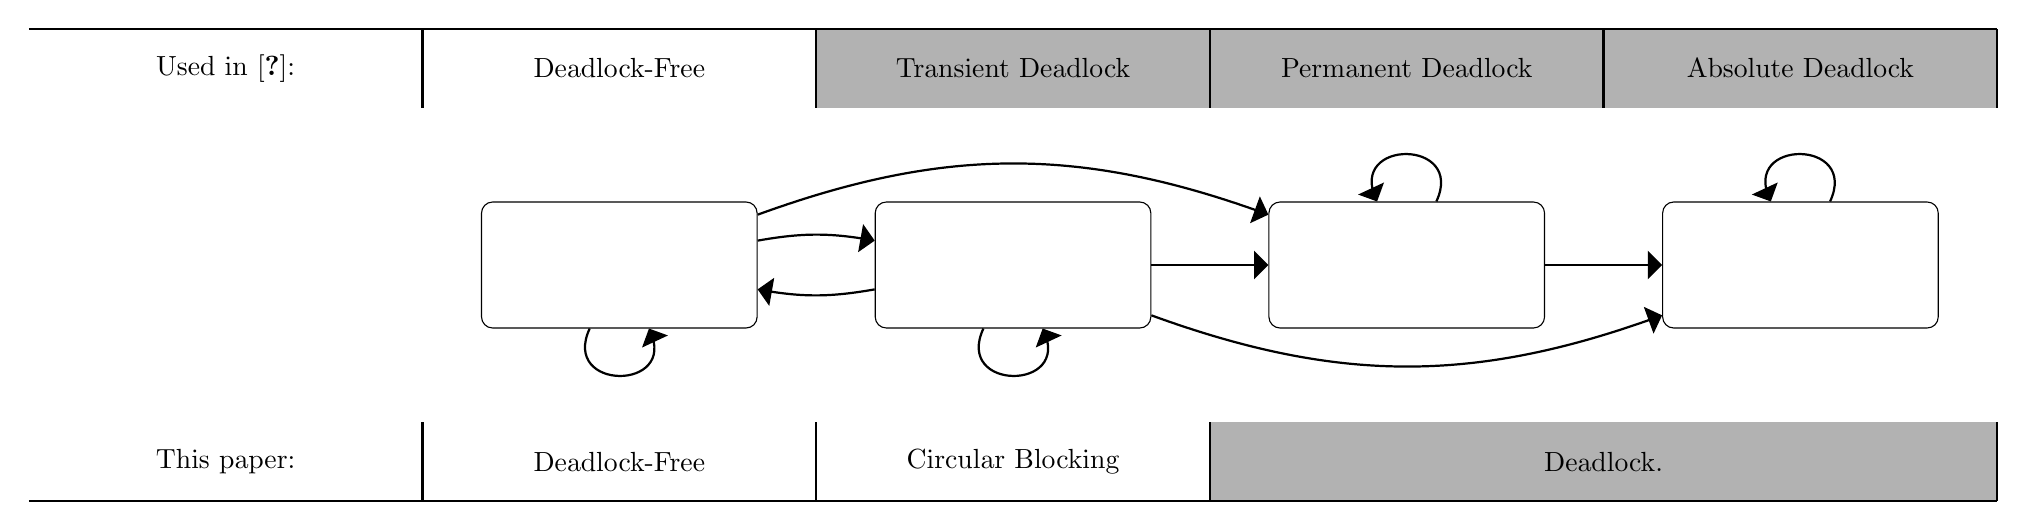
\begin{tikzpicture}

\node[align=center, draw=black, minimum height = 1.6cm, minimum width = 3.5cm, rounded corners] (deadlockfree) at (0, 0) {};
\node[align=center, draw=black, minimum height = 1.6cm, minimum width = 3.5cm, rounded corners] (circularblocking) at (5, 0) {};
\node[align=center, draw=black, minimum height = 1.6cm, minimum width = 3.5cm, rounded corners] (deadlock) at (10, 0) {};
\node[align=center, draw=black, minimum height = 1.6cm, minimum width = 3.5cm, rounded corners] (absolutedeadlock) at (15, 0) {};

\draw[thick, black, -triangle 90] (deadlockfree) [out=10, in=170, looseness=1] to (circularblocking);
\draw[thick, black, -triangle 90] (circularblocking) [out=-170, in=-10, looseness=1] to (deadlockfree);
\draw[thick, black, -triangle 90] (circularblocking) to (deadlock);
\draw[thick, black, -triangle 90] (deadlock) to (absolutedeadlock);
\draw[thick, black, -triangle 90] (deadlockfree) [out=20, in=160, looseness=1] to (deadlock);
\draw[thick, black, -triangle 90] (circularblocking) [out=-20, in=-160, looseness=1] to (absolutedeadlock);

\draw[thick, black, -triangle 90] (deadlockfree) [out=-115, in=-65, looseness=3] to (deadlockfree);
\draw[thick, black, -triangle 90] (circularblocking) [out=-115, in=-65, looseness=3] to (circularblocking);
\draw[thick, black, -triangle 90] (deadlock) [out=65, in=115, looseness=3] to (deadlock);
\draw[thick, black, -triangle 90] (absolutedeadlock) [out=65, in=115, looseness=3] to (absolutedeadlock);

\draw[draw=none, fill=black!30] (7.5, -2) rectangle (17.5, -3);
\draw[draw=none, fill=black!30] (2.5, 2) rectangle (17.5, 3);

\draw[thick, black] (-7.5, -3) -- (17.5, -3);
\draw[thick, black] (-2.5, -2) -- (-2.5, -3);
\draw[thick, black] (2.5, -2) -- (2.5, -3);
\draw[thick, black] (7.5, -2) -- (7.5, -3);
\draw[thick, black] (17.5, -2) -- (17.5, -3);

\node at (-5, -2.5) {This paper:};
\node at (0, -2.5) {Deadlock-Free};
\node at (5, -2.5) {Circular Blocking};
\node at (12.5, -2.5) {Deadlock.};

\draw[thick, black] (-7.5, 3) -- (17.5, 3);
\draw[thick, black] (-2.5, 2) -- (-2.5, 3);
\draw[thick, black] (2.5, 2) -- (2.5, 3);
\draw[thick, black] (7.5, 2) -- (7.5, 3);
\draw[thick, black] (12.5, 2) -- (12.5, 3);
\draw[thick, black] (17.5, 2) -- (17.5, 3);

\node at (-5, 2.5) {Used in \cite{venkateshetal98}:};
\node at (0, 2.5) {Deadlock-Free};
\node at (5, 2.5) {Transient Deadlock};
\node at (10, 2.5) {Permanent Deadlock};
\node at (15, 2.5) {Absolute Deadlock};


\end{tikzpicture}

\end{document}
